% !TeX spellcheck = en_US
\documentclass[12pt, a4paper,twoside]{report}
\title{Internship Report}
\author{Huu Duc Nguyen}
\date{February 2022}

\usepackage{acronym}
\usepackage{graphicx}
\graphicspath{{./Contents/images}}
\usepackage[utf8]{inputenc}
\usepackage[T1]{fontenc}
\usepackage[english]{babel}
\usepackage[final]{listings}
\usepackage{xcolor}
\usepackage{titlesec}
\usepackage{blindtext}
\usepackage{multicol}
\usepackage{geometry}
\geometry{a4paper, margin=0.9in}
\makeatletter
\usepackage[font=small]{caption}
\usepackage{xspace}
\usepackage{hyperref}
\usepackage{url}
\usepackage[backend=bibtex,style=alphabetic,]{biblatex}
\addbibresource{Contents/bibliography.bib}

%% the \onedot macro is producing only one dot at line ends.
%% thus \etal. will not produce et al..
\DeclareRobustCommand\onedot{\futurelet\@let@token\@onedot}
\def\@onedot{\ifx\@let@token.\else.\null\fi\xspace}
\def\eg{e.g\onedot} \def\Eg{E.g\onedot}
\def\ie{i.e\onedot} \def\Ie{I.e\onedot}
\def\cf{cf\onedot} \def\Cf{Cf\onedot}
\def\etc{etc\onedot} \def\vs{vs\onedot}
\def\wrt{w.r.t\onedot} \def\dof{d.o.f\onedot}
\def\figref#1{Fig.~\ref{#1}}

\def\citeaus#1{\citeauthor{#1} \cite{#1}}
\def\citeausm#1{\citeauthor*{#1} \cite{#1}}

\titleformat{\chapter}[block]%
{\bfseries\Large\filright}%
{\fontsize{27}{27}\selectfont\color{black}\thechapter}%
{1em}
{\fontsize{27}{50}\selectfont\scshape}%
[\vspace{-2ex}]

\begin{document}
\begin{titlepage}
	\begin{center}
		\begin{multicols}{2}
			
\includegraphics[width=0.35\textwidth]{bosch.png}\\
			%\textbf{Robert Bosch GmbH}\\
			Corporate Research / Advance Autonomous Systems (CR/AAS3)\\
			
\includegraphics[width=0.49\textwidth]{igmr.png}\\~\\
			%\textbf{RWTH Aachen University}\\
			%Institute of Mechanism Theory, Machine Dynamics and Robotics (IGMR)
		\end{multicols}	
		\vspace*{5cm}
		\large Robotic Systems Engineering\\
		\Huge \textbf{Internship Report}
		
		\vspace{2.5cm}
		\large
		\textit{Made by:}\\
		Huu Duc Nguyen\\
		\vspace*{1.5cm}
		\textit{Supervised by:}\\
		Robert Schirmer\\
		Marco Lampacrescia\\		
		\vfill		
		February, 2022
		
	\end{center}
\end{titlepage}

\section*{Acknowledgments}
I would like to thank the Robert Bosch GmbH for this opportunity, Robert Schirmer M.Sc. and Marco Lampacrescia M.Sc. for supervising and guiding me during this internship.
\clearpage

\tableofcontents
\clearpage
\section*{General abbreviations}
\addcontentsline{toc}{chapter}{{General abbreviations}}
\begin{acronym}[LONGEST]
	\acro{BASH}{Bourne Again SHell}
	\acro{CI}{Continuous Integration}
	\acro{CLI}{Conmand Line Interface}
	\acro{CPP}{Coverage Path Planning}
	\acro{CSP}{Covering Salemans Problem}
	\acro{EE}{End effector}
	\acro{PID}{Process identification number}
	\acro{POD}{Plain Old Data}
	\acro{PP}{Path Planning}
	\acro{ROS}{Robot Operating System}
	\acro{TSP}{Travelling Salemans Problem}
\end{acronym}

% !TeX spellcheck = en_US
\chapter{Introduction}

In the last semester of the robotic master program, there are two paths to follow: either focusing on academic research or gaining more industrial experience. With a desire to gain more hands-on experiences and skills, I decided to pursuit the industrial track, which requires a mandatory internship at an external company. I have already finished the master thesis at the Robert Bosch GmbH before the internship. Around the end of the thesis, my supervisors and I have discussed and agreed to continue on an 12-week internship.\\

Robert Bosch GmbH \cite{bosch}, also known as Bosch, is a multinational engineering and technology company. It was founded by Robert Bosch in 1886 in Stuttgart and currently is headquartered at Gerlingen. The company majors in four business sectors: Mobility Solutions, Industrial Technology, Consumer Goods, and Energy and Building Technology.\\

During the internship, I implemented additional features, which relate to my master thesis, into the department's robotic pipeline. The goal is to support the development of the next generation cleaning robot. This report summarizes what I have learn during the time spending at the company.
\clearpage
% !TeX spellcheck = en_US
\chapter{Coding Languages And Tools}

Across the time working on the thesis and the internship, I had the opportunity to experience the professional workflow with state-of-the-art methods. This section summarizes common languages, tools for developers and the workflow. In addition the presented languages and tools, I also either worked with or got to know more about Docker \cite{merkel2014docker}, Python, Vim, git, \etc.

\section{Bash}

\subsection{Introduction}

Linux is a family of operating systems based on the Linux kernel. For public users, it is less common and well-known comparing to Windows and Mac. These two receive more attention for application developments, however, give little access to the source code and are more prone to malware. On the other hands, Linux is open-source and enables more accesses to modify the system configurations. For engineers and developers, Linux induces a better working environment.\\

\ac{BASH} is a Unix shell and command language. It is the default login shell for most Linux distributions. Bash allows users to interact with the operating system, accessing, managing file system.

\subsection{Basic commands}

Developers would spend a significant part of his time working in the \ac{CLI}. It is important to familiarize themselves with common \ac{BASH}/Shell commands and programs:

\begin{itemize}
	\setlength\itemsep{0em}
	\item View the file system: \verb|ls, tree|, \texttt{broot} \cite{broot}, \texttt{exa} \cite{exa}, \texttt{ranger} \cite{ranger}.
	
	Working in a coding project, developers would find themselves going through either existing or green field file system. It is crucial to know what files or directories there are, their positions, whether one could read, write or execute the files, \etc. \texttt{ls} and \texttt{tree} are the basic commands to view the file system and related information. \texttt{broot, exa} and \texttt{ranger} are more advanced commands with more features, \eg, color coding, interactive actions (change directory, move, delete files, \etc). Files and directories have permissions, which can be view from the long descriptions. "d" implies directory, otherwise "." implies a file. The next 9 characters show the permissions of three groups, \ie, owner, owning group and everyone else. Each group could have 3 permissions: "r" read, "w" write and "x" execute. In addition, these commands could display information regarding file size, file owner, modified date, git tracking status (if available).
	\begin{figure}[hbt!]
		\centering
		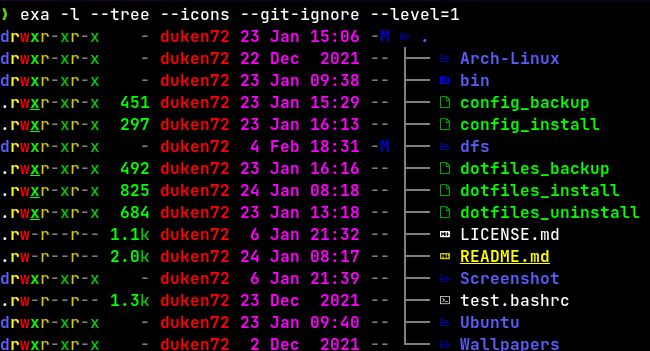
\includegraphics[width=0.9\textwidth]{exa.png}
		\caption{Viewing file system with \texttt{exa}.}
	\end{figure}

	\item View files or directories descriptions: \verb|file, du|, \verb|cloc| \cite{cloc}, \verb|tokei| \cite{tokei}
	
	\verb|file| - determine file type, \verb|du| - estimate file space usage, \verb|cloc| - count lines of code, \verb|tokei| - display statistics about your code. Some additional info regarding number of code lines, files, file and directory memory size, comments, \etc, is also needed. These info can be accessed and included with these commands. Example of \texttt{tokei}:
	\begin{verbatim}
	================================================================
	Language        Files    Lines     Code    Comments     Blanks
	================================================================
	BASH                8      118       85          14         19
	C Header           26     1871      986         528        357
	C++                16     3373     2627         326        420
	Makefile            2       60       38           4         18
	Python              1      173      110          36         27
	Shell               4     1669     1392         162        115
	Plain Text          4       98        0          86         12
	Zsh                14    20719    13838        5146       1735
	----------------------------------------------------------------
	Markdown            8     2998        0        2225        773
	|- BASH             3      119      103           6         10
	|- C++              1      137      132           0          5
	|- Lua              2        8        8           0          0
	|- YAML             2        6        6           0          0
	|- Zsh              3      167      136          20         11
	(Total)                   3435      385        2251        799
	================================================================
	Total              83    31079    19076        8527       3476
	================================================================
	\end{verbatim}
	
	\item Change ownership, permission: \verb|chown|, \verb|chmod|.
	
	\verb|chown| - change file or directory ownership, \verb|chmod| - change file or directory permissions.
	\item Search for file: \verb|locate, find|, \verb|fdfind| \cite{fdfind}, \verb|fzf| \cite{fzf}.
	
	\verb|locate| - list files in databases that match a pattern, \verb|find| - search for files in a directory hierarchy, \verb|fdfind| - user-friendly alternative to \texttt{find}, \verb|fzf| - a general-purpose command-line fuzzy finder.
	\begin{figure}[hbt!]
		\centering
		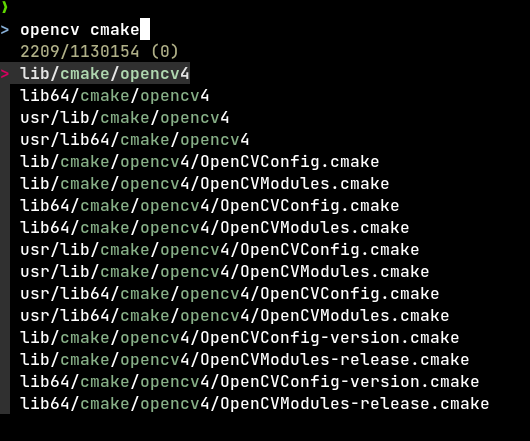
\includegraphics[width=0.9\textwidth]{fzf.png}
		\caption{Searching for file with fuzzy finder \texttt{fzf}.}
	\end{figure}
	\item Read guidance: \verb|man|, \verb|which|, \verb|apropos|, \verb|type|.
	
	\verb|man| - an interface to the system reference manuals, \verb|which| - shows the full path of (shell) commands, \verb|apropos| - search the manual page names and descriptions, \verb|type| - write a description of command type.
	
	\item Manage files and directories: \verb|mkdir|, \verb|rmdir|, \verb|touch|, \verb|cp|, \verb|mv|, \verb|rm|, \verb|ln|.
	
	\verb|mkdir| - make directories, \verb|rmdir| - remove empty directories, \verb|touch| - change file timestamps, \verb|cp| - copy files and directories, \verb|mv| - move (rename) files, \verb|rm| - remove files or directories, \verb|ln| - make links between files.
	
	\item View file content: \verb|cat, more, less|, \verb|bat| \cite{bat}.
	
	\verb|cat| - concatenate files and print on the standard output, \verb|more| - file filter for paging through text one screenful at a time, \verb|less| - provide \verb|more| emulation plus extensive enhancements, \verb|bat| - a \verb|cat| clone with syntax highlighting and Git integration.
	
	\item Edit file content: \verb|nano|, \verb|gedit|, \verb|vi|, \verb|vim|, \verb|sed|, \verb|sd| \cite{sd}, \verb|awk|, or file-specific application.
	
	Example commands for \texttt{sd} and \texttt{sed}:
	\begin{verbatim}
		sd [prev_expression] [new_expression] [file]
		sd [prev_expression] [new_expression] [file] -p #p-preview
		# just print out the results
		sed 's/[prev_expression]/[new_expression]/g' [file.txt]
		# replace a string with another
		sed -i 's/[prev_expression]/[new_expression]/g' [file.txt]
		sed '/searchStr/c\newLine' [file.txt] # replace a line contain a string
		
		awk '/pattern/ {print $2}' file.txt
		awk -f awkFD.awk file.txt
	\end{verbatim}
	
	\item Archive: \verb|zip|, \verb|unzip|, \verb|zipcloak|, \verb|zipslit|, \verb|tar|, \verb|gzip|, \verb|gunzip|, \verb|unrar|.
	
	\verb|zip| - package and compress (archive) files, \verb|unzip| - list, test and extract compressed file in a ZIP archive, \verb|zipcloak| - encrypt entries in a ZIP file, \verb|zipslit|, \verb|tar| - an archiving utility, \verb|gzip|, \verb|gunzip| - compress and expand files, \verb|unrar| - uncompress RAR archive .
	
	Some of the tags for \texttt{zip} are: \texttt{-r} for recursive search, \texttt{-e} for encryption, \texttt{-v} for more verbose output, \texttt{-9} for better compression. Example of recursive compression with encryption:
	\begin{verbatim}
		zip -er9 output.zip file1 file2
	\end{verbatim}
	Some tags for \texttt{unzip} are: \texttt{-x} for files exclusion, \texttt{-o} for overwrite, \texttt{-n} for not-overwrite, \texttt{-d} for output directory, \texttt{-l} for listing content. Examples of uncompress a \texttt{.zip} file:
	\begin{verbatim}
		unzip -o input.zip -x *.h -d target_dir
		upzip -l input.zip
	\end{verbatim}
	Additional commands for \texttt{.zip} files:
	\begin{verbatim}
		zipcloack file.zip # add password
		zipsplit -n [size_in_bytes] file.zip # split to size restriction
	\end{verbatim}
	Some tags for \texttt{tar}: \texttt{v} for more verbose output, \texttt{f} for files, \texttt{c} for create, \texttt{z} for \texttt{.gunzip} file, \texttt{x} for extract, \texttt{t} for listing. Examples of \texttt{tar} commands:	
	\begin{verbatim}
		tar cvf [target_file.tar] [files/dirs] # create .tar
		tar zcvf [target_file.tar.gz] [files/dirs] # create .tar.gz
		tar tvf [file.tar] # list out files in file.tar
		tar xvf [file.tar] -C [dirs] # extract tar file
		tar xvfz [file.tar.gz] [dirs] # extract tar.gz file
	\end{verbatim}
	
	Other commands with \verb|gzip, gunzip, unrar| for archiving and compression:
	\begin{verbatim}		
		gzip [file.tar] # compress the tar file to .tar.gz file
		gunzip [file.tar.gz] # uncompress the .tar.gz file to .tar file
		unrar x [file.rar]
	\end{verbatim}
	
	\item Monitor your system: \verb|htop|, \verb|neofetch|
	
	\texttt{htop} is the equivalent Linux-version of Task Manager in Windows, from which user can inspect current running process, application, in terms of memory, CPU percentages, end a process if desired.
	\begin{figure}[hbt!]
		\centering
		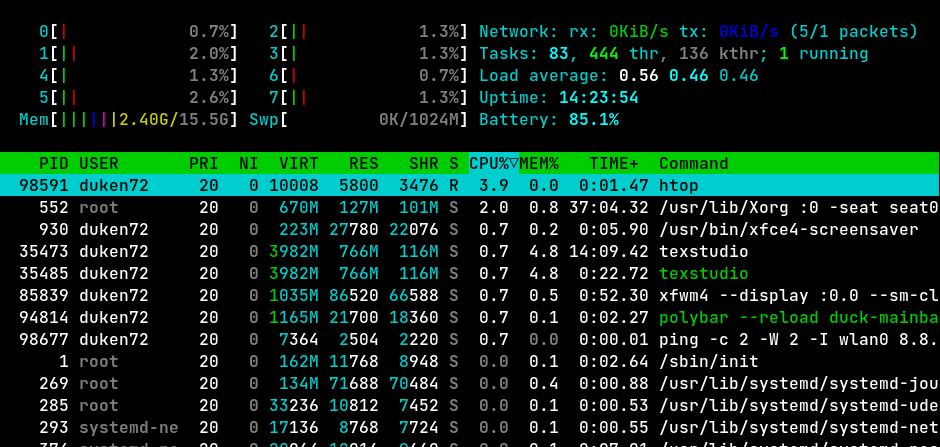
\includegraphics[width=0.9\textwidth]{htop.png}
		\caption{System inspection with \texttt{htop}.}
	\end{figure}
	\begin{figure}[hbt!]
		\centering
		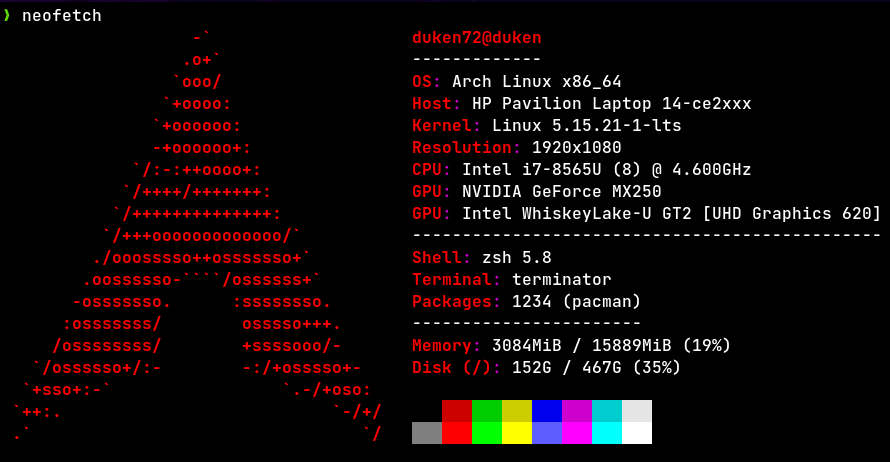
\includegraphics[width=0.9\textwidth]{neofetch.png}
		\caption{System inspection with \texttt{neofetch}.}
	\end{figure}

	\item Cryptography: \verb|openssl|
	
	Example commands:
	\begin{verbatim}
		openssl aes-256-cbc -salt -pbkdf2 -in <file.name> -out <file.enc.name>
		openssl aes-256-cbc -d -pbkdf2 -in <file.enc.name> -out <file.dec.name>
		cmp <file1> <file2> | echo \$? \#compare 2 file, 0 if same, 1 if different	
	\end{verbatim}
	\item Managing working processes: \verb|fg|, \verb|bg|, \verb|jobs|, \verb|kill|.
	
	\verb|fg| - run jobs in the foreground, \verb|bg| - run jobs in the background, \verb|jobs| - display status of jobs in the current session, \verb|kill| - terminate a process.	
\end{itemize}

\subsection{Shell scripting}

As a scripting language, user-defined aliases and programs could incorporate different basic commands. On top of a Shell program, the shebang must be included: \verb|#!/bin/sh| or \verb|#!/bin/bash|. The Shell language allows defining variables, accessing arguments, logical operator, flow control, etc.

\subsubsection{Variables to access}

The variables are accessed via \verb|$| sign.
\begin{itemize}
	\setlength\itemsep{0em}
	\item \verb|$0| - Name of the script
	\item \verb|$1| to \verb|$9| - Arguments to the script. \verb|$1| is the first argument and so on.
	\item \verb|$@| - All the arguments
	\item \verb|$#| - Number of arguments
	\item \verb|$?| - Return code of the previous command
	\item \verb|$$| - \ac{PID} for the current script
	\item \verb|!!| - Entire last command, including arguments, \eg: \verb|sudo !!| if last command fail due to permission
	\item \verb|$_| - Last argument from the last command.
\end{itemize}

\subsubsection{Logical operators}
There are three logical operators:
\begin{itemize}
	\setlength\itemsep{0em}
	\item The \texttt{||} operator:
	\begin{verbatim}
		false || echo "Oops, fail" # Oops, fail
		true || echo "Will not be printed"
	\end{verbatim}
	\item The \verb|&&| operator acts like an \texttt{AND} operator:
	\begin{verbatim}
		true && echo "Things went well" # Things went well
		false && echo "Will not be printed"		
	\end{verbatim}
	\item The \texttt{;} operator acts like an \texttt{OR} operator:
	\begin{verbatim}
		true ; echo "This will always run"
		false ; echo "This will always run"
	\end{verbatim}
\end{itemize}

\subsubsection{Flow controls}
With \ac{BASH}, there are flow controls just like in common languages, \eg, Python or C++.
\begin{itemize}
	\setlength\itemsep{0em}
	\item If-else statement:
	\begin{verbatim}
		if conditions; then
		  commands
		[elif conditions; then
		  commands]
		[else conditions; then
		  commands]
		fi
		
		# Multiple conditions:
		if ([condition1] || [condition2]) && [condition3]; then
		  commands
		fi
	\end{verbatim}
		
	\item For loop:
	\begin{verbatim}
		for i in word1 word2 word3; do
		  echo "$i"
		done
		
		for i in "$@"; do
		  echo $i
		done
	\end{verbatim}
	\item While loop:
	\begin{verbatim}
		while [ condition ] do
		  command1
		  command2
		  command3
		done
	\end{verbatim}
	
\end{itemize}

\subsubsection{Comments}
\begin{itemize}
	\setlength\itemsep{0em}
	\item Single line comments with "\verb|#|"\\
	Example: \verb|# Flow Control|
	\item Block comments
	\begin{verbatim}
	: <<'END'
	echo "I hope that there is no error"
	END
	\end{verbatim}
\end{itemize}

\subsubsection{Logic conditions}

Common logical conditions relate with file system. There are syntax to check whether a file exists and is of the expected type.

\begin{verbatim}
	if [ -d file ]; then echo "file is a directory" fi
	if [ -e file ]; then echo "file exists" fi
	if [ -f file ]; then echo "file exists and is a regular file" fi
	if [ -L file ]; then echo "file is a symbolic link" fi
	if [ -r file ]; then echo "file is a file readable by you" fi
	if [ -w file ]; then echo "file is a file writable by you" fi
	if [ -x file ]; then echo "file is a file executable by you" fi
	if type cmd; then echo "cmd exists" fi
	
	if [ file1 -nt file2 ]; then echo "file1 is newer than file2" fi
	if [ file1 -ot file2 ]; then echo "file1 is older than file2" fi
\end{verbatim}

In addition, there are syntax logic conditions to comparison between \texttt{string}:
\begin{verbatim}
	if [ -z string ]; then echo "string is empty" fi
	if [ -n string ]; then echo "string is not empty" fi
	if [ string1 = string2 ]; then echo "string1 equals string2" fi
	if [ string1 != string2 ]; then echo "string1 does not equal string2" fi
\end{verbatim}

\subsection{CLI Hotkeys}

It is useful to practice and remember some basic hotkeys while working on the \ac{CLI}. It should noted that different shells have different features regarding line completion and movements.

\begin{table}[hbt!]
	\centering
	\begin{tabular}{c|c}
		Commands   & Actions                           \\
		\hline\hline
		\verb|CTRL-A / E| & move to home/end of line       \\
		\verb|CTRL-F / B| & move for/backward a character   \\
		\verb|ALT -F / B| & move for/backward a word   \\
		\verb|CTRL-H| & delete char                  \\
		\verb|CTRL-W| & delete a word back             \\
		\verb|CTRL-K| & clear to end of line\\
		\verb|CTRL-U| & clear the line                   \\
		\verb|CTRL-S / Q| & toggle screen output       \\
		\verb|CTRL-L| & clear screen output            \\
		\verb|Ctrl-D| & exit shell                     \\
		\verb|CTRL-C| & stop current process          
	\end{tabular}
\end{table}

\section{CMake}

\subsection{Introduction}
CMake is a tool for build system, usually for projects or programs written in C or C++ language. Programmers write and work with source code. However, in order for the computers to understand and execute those programs, the source code needs to be built (compile and link with libraries) into binary file. Previously, \texttt{Makefile}s compile and build the source code, thus there is a need to maintain and update these \texttt{Makefile}s. As the project scale grows, this maintaining and updating tasks become more tedious. \Eg, when working with ROS, current package might use multiple external packages and libraries, which could have more than one executable, different build and test configurations. Build tools like CMake are developed to automate the complex build process. Instead of manually manage \texttt{Makefile}s, developers manage \texttt{CMakeLists.txt} file, which will create \texttt{Makefile}s. This section gives an overview on CMake.\\

\subsection{CMake Syntax}
CMake has its own scripting language, which includes variables, statements, flow control, commands, \etc. Some basic commands, syntax are as follows:
\begin{itemize}
	\setlength\itemsep{0em}
	\item Print message
	
	\verb|message("Hello world!")     # Print "Hello world!"|\\
	\verb|message("Hello ${NAME}!")   # Substitute a variable into the message|
	\item Assign variables
	
	\texttt{set(THING duck)}\\
	\verb|message("We want the ${THING}!")|
		
	In CMake, every variables are strings, which in most case relate to paths, names of files, libraries or configurations.
	\item Math operation
	
	\verb|math(EXPR MY_SUM "1 + 1")    # Store 2 in MY_SUM|\\
	\verb|message("The sum is ${MY_SUM}.")|	
	\item Flow control
	\begin{itemize}
		\item If-else statement
		\begin{verbatim}
			if(WIN32)
			  message("You're running CMake on Windows.")
			else()
			  message("You're not running CMake on Windows.")
			endif()
		\end{verbatim}
		\item While loop
		\begin{verbatim}
			set(A "1")
			set(B "1")
			while(A LESS "7")
			  message("A = ${A}")         # Print A
			  math(EXPR T "${A} + ${B}")  # Store the sum of A and B in T
			  set(A "${B}")               # Assign the value of B to A
			  set(B "${T}")               # Assign the value of T to B
			endwhile()
		\end{verbatim}
		\item For loop
		\begin{verbatim}
			foreach(ARG These are separate arguments)
			  message("${ARG}")       # Prints each word on a separate line
			endforeach()
		\end{verbatim}
		
	\end{itemize}	
	\item Combine commands with variable:
	\begin{verbatim}
		set(ARGS "EXPR;T;1 + 1")
		math(${ARGS})   # Equivalent to math(EXPR T "1 + 1")
		message("${ARGS}")
	\end{verbatim}
	\item List
	\begin{verbatim}
		set(MY_LIST These are separate arguments)
		message("${MY_LIST}")
		# Prints: These;are;separate;arguments
		
		set(MY_LIST These are separate arguments)
		list(REMOVE_ITEM MY_LIST "separate")
		# Removes "separate" from the list
		message("${MY_LIST}")
	\end{verbatim}
	\item Function
	\begin{verbatim}
		function(doubleIt VALUE)
		  math(EXPR RESULT "${VALUE} * 2")
		  message("${RESULT}")
		endfunction()
		
		# Prints: 8
		doubleIt("4")
	\end{verbatim}
	\item Marco
	\begin{verbatim}
		macro(doubleIt VARNAME VALUE)
		  # Set the named variable in caller's scope
		  math(EXPR ${VARNAME} "${VALUE} * 2")
		endmacro()
		
		# Tell the macro to set the variable named RESULT
		doubleIt(RESULT "4")					
		
		# Prints: 8
		message("${RESULT}")					
	\end{verbatim}
\end{itemize}

\subsection{CMake Target and Properties}
Targets are executable files, binary files. As the name itself suggests, they are the targets, the goal of CMake, to compile and build source code (in C++) to these executables. In other cases, instead of executable(s), the targets to build could be libraries, which are groups of functionalities that could be used somewhere else. The commands to define these targets are:
\begin{itemize}
	\setlength\itemsep{0em}
	\item \verb|add_executable|: define the target
	\item \verb|add_subdirectory, add_library, add_custom_target|: call \verb|CMakeLists.txt| from lower directory level.
\end{itemize}

These executables have properties, which are to be managed in order for the source code to be compiled and linked properly. Some common properties are:
\begin{itemize}
	\setlength\itemsep{0em}
	\item \verb|INCLUDE_DIRECTORIES|
	
	Include directories are where to find the C++ header files. With correct paths, header files can be included on top of the \verb|.cpp| files: \verb|#include <something.h>|. This is where the compiler will find function declarations, type definitions, classes, structures, \etc.
	\item \verb|LINK_LIBRARIES|
	
	While compiler concerns with the declarations, linker concerns with functions, methods definitions. These are handled by link libraries. In the build process, a target has to be compiled and linked in order to become a executable.
	\item \verb|COMPILE_DEFINITIONS|
	\item \verb|COMPILE_OPTIONS|
\end{itemize}

The commands to change or update these properties:

\begin{itemize}
	\setlength\itemsep{0em}
	\item \verb|(target_)include_directories|
	\item \verb|(target_)link_libraries|
	\item \verb|(target_)compile_definitions|
	\item \verb|(target_)compile_options|
	\item \verb|set_property|
	\item \verb|get_property|
\end{itemize}

For example, the following line gets the the \verb|SOURCES| property of the target \texttt{MyApp} and assigns it to \verb|MYAPP_SOURCES|:

\verb|get_property(MYAPP_SOURCES TARGET MyApp PROPERTY SOURCES)|

\subsection{Build Types}

There are different build types:
\begin{itemize}
	\setlength\itemsep{0em}
	\item \verb|Release|: high optimization level, no debug info, code or asserts.
	\item \verb|Debug|: No optimization, asserts enabled, custom debug (output) code enabled, debug info included in executable (so you can step through the code with a debugger and have address to source-file:line-number translation).
	\item \verb|RelWithDebInfo|: optimized, with debug info, but no debug (output) code or asserts.
	\item \verb|MinSizeRel|: same as Release but optimizing for size rather than speed.
\end{itemize}

In case of missing \verb|FindPackage.cmake| error, one could search for customized script online and put it in the package directory as follow:

\begin{figure}[hbt!]
	\centering
	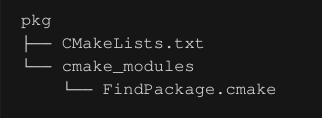
\includegraphics[width=0.7\textwidth]{findPackageCmake.png}
\end{figure}

In the top-level \verb|CMakeLists.txt|, add this line before \verb|find_package|:\\

\verb|list(APPEND CMAKE_MODULE_PATH ${CMAKE_CURRENT_LIST_DIR}/cmake_modules)|

\section{C++}
C++ is a statically typed programming language. On the other hand, Python is a dynamically typed programming language, which implies that developers don't have to think and define the type of all variables with care. C++ allows low-level memory and hardware control like the C language, but with high-level abstraction with classes and structures. With its computational and memory efficiency, the language has usage in game engines, databases, embedded systems, desktop software, \etc. When working with \ac{ROS}, the coding languages are C++ and Python. However, for most real-time operations and features, C++ is more preferable.

\subsection{Memory Management and Pointer}

\subsubsection{Variable types and sizes}

The primitive data types vary in the memory size that they occupy. Be aware that sometimes, the actual memory size also depends on the compiler or the data models. In addition, there are modifiers to the type:

\begin{itemize}
	\setlength\itemsep{0em}
	\item Signedness
	 \begin{itemize}
	 	\setlength\itemsep{0em}
		\item \verb|signed| (default) - have signed representation, loosing 1 bit
		\item \verb|unsigned| - have unsigned representation
	\end{itemize}
	\item Size \begin{itemize}
		\setlength\itemsep{0em}
		\item \verb|short| - be optimized for space and will have width of at least 16 bits.
		\item \verb|long| - have width of at least 32 bits.	
	\end{itemize}
\end{itemize}

\begin{table}[htb!]
	\centering
	\begin{tabular}{rcc}
		\textbf{Type}          & \textbf{Size}     & \textbf{Typical Range}   \\
		\hline\hline
		boolean                & 8 bits = 1 byte   & $0-1$                    \\
		(signed) char          & 8 bits = 1 byte   & $-2^7$ to $2^7-1$        \\
		unsigned char          & 8 bits = 1 byte   & $0$ to $2^8-1$           \\
		(signed) int           & 32 bits = 4 bytes & $-2^{31}$ to $2^{31}-1$  \\
		unsigned int           & 32 bits = 4 bytes & $0$ to $2^{32}-1$        \\
		(signed) short int     & 16 bits = 2 bytes & $-2^{15}$ to $2^{15}-1$  \\
		unsigned short int     & 16 bits = 2 bytes & $0$ to $2^{16}-1$        \\
		(signed) long int      & 32 bits = 4 bytes & $-2^{31}$ to $2^{31}-1$  \\
		unsigned long int      & 32 bits = 4 bytes & $0$ to $2^{32}-1$        \\
		(signed) long long int & 64 bits = 8 bytes & $-2^{63}$ to $2^{63}-1$  \\
		unsigned long long int & 64 bits = 8 bytes & $0$ to $2^{64}-1$        \\
		float                   & 32 bits = 4 bytes & $3.4E\pm38$ (7 digits)   \\
		double                 & 64 bits = 8 bytes & $1.7E\pm308$ (15 digits)
	\end{tabular}
	\caption{Data types with their size and range.}
\end{table}

A \verb|boolean| just needs 1 bit, but you can only access byte, thus it still occupies 1 byte, which is 8 bits. We could however store 8 \verb|bool|(s) in 1 byte. Suffixes are used to differentiate types when assigning variables. These suffixes are case-insensitive: \ie, `u` is equivalent to `U`, `UL` is equivalent to `uL, Ul, ul`.

\begin{table}[htb!]
	\centering
	\begin{tabular}{ccc}
		\textbf{Data Type} & \textbf{Suffix}   & \textbf{Meaning}   \\
		\hline\hline
		int                & U               & unsigned int       \\
		int                & L               & long               \\
		int                & UL / LU         & unsigned long      \\
		int                & LL              & long long          \\
		int                & ULL / LLU       & unsigned long long \\
		double             & F               & float               \\
		double             & L               & long double       
	\end{tabular}
	\caption{Suffixes for data types.}
\end{table}

\subsubsection{Stack and Heap Memory}

Allocating on the stack is fast, simple as only one CPU commands. There is a lot happen behind the scene when assigning a value on heap memory. To find the free space, assign, book keeping, .. In case you have something very memory heavy, then you have to use the heap.

\begin{itemize}
	\setlength\itemsep{0em}
	\item Allocate with the stack:\\
	\verb|int value = 5;|	
	\item Allocate with the heap:\\
	\verb|int* hvalue = new int;|\\
	\verb|*hvalue = 5;|
\end{itemize}

\subsubsection{new and delete operator}

The \verb|new| operator does two things: allocating memory and calling the constructor. The main purpose of \verb|new|, is to allocate memory, on the HEAP specifically. The \verb|delete| operator calls the destructor and then frees the memory.

Additional notes:
\begin{itemize}
	\setlength\itemsep{0em}
	\item Arrays created with \verb|new []| must be destroyed with \verb|delete[]|.
	\item Using \verb|new|, the object created remains in existence until you \verb|delete| it. Without using \verb|new|, the object will be destroyed when it goes out of scope.
	\item Every time you type \verb|new|, type \verb|delete|.
\end{itemize}

\subsubsection{Smart Pointers}

Unconscious not deallocating a pointer causes a memory leak that may lead to crash of the program. For languages with Garbage Collection Mechanisms to smartly deallocate unused memory, \eg, Java and C\#, programmers don't have to worry about memory leak. C++11 comes up with its own mechanism: Smart Pointer. When the object is destroyed, it frees the memory as well.

With \verb|#include <memory>|:
\begin{itemize}
	\setlength\itemsep{0em}
	\item \verb|std::unique_ptr| stores one pointer only. We can assign a different object by removing the current object from the pointer.
	\item \verb|std::shared_ptr| allows more than one pointer pointing to this one object at a time and it’ll maintain a Reference Counter using \verb|use_count()| method.
	\item \verb|std::weak_ptr| also allows more than one pointer pointing at one object at a time, but without a Reference Counter.
	\item \verb|std::auto_ptr| is replaced by \verb|std::unique_ptr|, with similar functionality, improved security, added features and support for arrays.
\end{itemize}

Good practice is to use \verb|std::make_shared| as a simple and more efficient way to create an object and a \verb|std::shared_ptr| to manage shared access to the object at the same time.

Let look into an example with these smart pointers. Assuming we have a \texttt{class A} with a simple method \texttt{show()}:
\begin{verbatim}
#include <memory>
#include <iostream>

class A
{
public:
  void show()
  {
    std::cout << "Run A::show()" << std::endl;
  }
};
\end{verbatim}

Initially, we can define also \verb|std::auto_ptr|. After C++11, this is depreciated.
\begin{verbatim}
int main()
{
  std::auto_ptr<A> p1(new A);
  p1->show();
  std::cout << "Memory address of p1 " << p1.get() << std::endl;
  std::auto_ptr<A> p2(p1);
  p2->show();
  std::cout << "Memory address of p1 " << p1.get() << std::endl;
  std::cout << p2.get() << std::endl;
}
\end{verbatim}

Example define and use \verb|std::unique_ptr|:
\begin{verbatim}
int main()
{
  std::unique_ptr<A> p1(new A);
  p1->show();
  std::cout << "Memory address of p1 " << p1.get() << std::endl;
}
\end{verbatim}

Since \verb|std::unique_ptr| allows only one pointer, attempt to copy will lead to error. The only way is to transfer the ownership
\begin{verbatim}
// Error: can't copy unique_ptr
// std::unique_ptr<A> p2 = p1;

// transfers ownership to p2
std::unique_ptr<A> p2 = move(p1);
p2->show();
std::cout << "Memory address of p1 " << p1.get() << std::endl;
std::cout << "Memory address of p2 " << p2.get() << std::endl;
std::cout << std::endl;
\end{verbatim}
Example create and use \verb|std::shared_ptr|

\begin{verbatim}
int main()
{
  std::cout << "smart_ptr example:" << std::endl;
  std::shared_ptr<A> p3(new A);
  std::cout << "Memory address of p3 " << p3.get() << std::endl;
  p3->show();
  std::shared_ptr<A> p4(p3);
  p4->show();
  std::cout << "Memory address of p3 " << p3.get() << std::endl;
  std::cout << "Memory address of p4 " << p4.get() << std::endl;  
  // Returns the number of shared_ptr objects
  // referring to the same managed object.
  std::cout << "Counts: " << p3.use_count() << std::endl;
  std::cout << "Counts: " << p4.use_count() << std::endl;
  // Relinquishes ownership of p1 on the object
  // and pointer becomes NULL
  p3.reset();
  std::cout << "Memory address of p3 " << p3.get() << std::endl;
  std::cout << "Counts: " << p4.use_count() << std::endl;
  std::cout << "Memory address of p4 " << p4.get() << std::endl;
  std::cout << std::endl;
}
\end{verbatim}

In practice, it is better to create this pointers with \verb|std::make_shared| or \verb|std::make_unique|
\begin{verbatim}
int main()
{
  // Good practice
  std::shared_ptr<A> p5 = std::make_shared<A>();
  std::unique_ptr<A> p5 = std::make_unique<A>();
}
\end{verbatim}

\subsection{Class Features}

\subsubsection{Constructor member initializer lists}

Normal constructor initialization:
\begin{verbatim}
Something::Something(int memIn1, double memIn2)
{
  mem1 = memIn1;
  mem2 = memIn2;
  mem3 = 'c';
};
\end{verbatim}


There are cases that initialization of data members inside constructor doesn’t work and Initializer List must be used: non-static constant data members, reference members, performance reasons, avoid unnecessary call to a default constructor, \etc. Initializing member values with initializer lists is better. The initializer list is inserted after the constructor parameters, after the ":" and separated by a ",".
\begin{verbatim}
Something::Something(int memIn1, double memIn2)
: mem1{memIn1}, mem2{memIn2}, mem3{'c'} {};
\end{verbatim}

\subsubsection{Structure versus Class}

Some features to differentiate between the use of structure and class in C++:

\textbf{Structure:}
\begin{itemize}
	\setlength\itemsep{0em}
	\item Default access specifier will be \verb|public|.
	\item The instance of the structure is known as "Structure variable".
	\item A \verb|struct| is a bundle of several related elements, which needed to be tied up together in a certain context. When a collection of \ac{POD} is needed.
\end{itemize}

\textbf{Class:}
\begin{itemize}
	\setlength\itemsep{0em}
	\item Default access specifier will be \verb|private|.
	\item The instance of the class is known as Object of the class.
	\item A \verb|class| can do things with its methods and members.
	\item Operators to work on new data type can be defined using special methods (over-loading operators).
	\item One class can be used as the basis for definition of another. If you use inheritance, don't use \verb|struct|, use \verb|class|.
	\item Declaration of a var of the new class type requires just the name of the class: \verb|classA varA;|, not: \verb|struct structA varA;|
\end{itemize}

\subsubsection{Virtual and Override Specifier}

These two concerns with Runtime Polymorphism. Without \verb|virtual|, you get early binding. With \verb|virtual|, you get late binding.

\begin{verbatim}
class Base
{
public:
  void Method1() { std::cout << "Base::Method1" << std::endl; }
  virtual void Method2() { std::cout << "Base::Method2" << std::endl; }
};

class Derived : public Base
{
public:
  void Method1() { std::cout << "Derived::Method1" << std::endl; }
  void Method2() { std::cout << "Derived::Method2" << std::endl; }
};

Base* basePtr = new Derived ();
//  Note - constructed as Derived, but pointer stored as Base*
basePtr->Method1();  //  Prints "Base::Method1"
basePtr->Method2();  //  Prints "Derived::Method2"
\end{verbatim}

In the above example, \texttt{Method1()} is defined without \texttt{virtual} specifier, thus, when we call \texttt{basePtr->Method1();}, the early binding calls the definition from the \texttt{Base} class. On the other hands, \texttt{Method2()} is defined in the \texttt{Base} class with \texttt{virtual} specifier, which implies late binding. Therefore, when \texttt{basePtr->Method2();} is called, the method of the \texttt{Derived} class is called.\\

When using \verb|virtual| functions, it is possible to make mistakes while declaring the member functions of the derived classes. Using the \verb|override| identifier prompts the compiler to display error messages when these mistakes are made.

\begin{verbatim}
class Base
{
public:
  virtual void Method2() { std::cout << "Base::Method2" << std::endl; }
};

class Derived : public Base
{
public:
  // override identifier will give Error for miss-typing Metod2
  void Metod2() { std::cout << "Derived::Method2" << std::endl; } override
};
\end{verbatim}

\subsection{Best practices and tips}

\subsubsection{Inline Specifier}

Inlining concerns with the overhead cost for switching time of small functions. When the \verb|inline| function is called, the whole code of the \verb|inline| function gets inserted or substituted. This substitution is performed by the C++ compiler at compile time. Inlining is only a request to the compiler, not a command. There are cases that the compiler can ignore this request. \verb|inline| functions have advantages but also disadvantages.
\begin{verbatim}
inline int cube(int s)
{
  return s*s*s;
}
\end{verbatim}

For Class definition, you only need to add \verb|inline| when defining it, not when declaring it inside the class.

\subsubsection{Explicit Specifier}

Specifies that a constructor or conversion function (since C++11) or deduction guide (since C++17) is \verb|explicit|, that is, it cannot be used for implicit conversions and copy-initialization. Example of implicit specifier:
\begin{verbatim}
class A
{
public:
  A();
  A(int);
  A(const char*, int = 0);
};

int main()
{
  A c = 1;
  A d = "Venditti";
}
\end{verbatim}

In this example, though variable \texttt{c} is of \texttt{class A}, which is not an \texttt{int}, it is okay to write initialize \texttt{A c = 1;} due to implicit conversion. The same happens with \texttt{A d = "Venditti";}. The above program exits without error.\\

However, the above usage might lead to accidental construction that can hide bugs. Thus, we might want to turn off the implicit conversion with \texttt{explicit} specifier. Example of explicit specifier:
\begin{verbatim}
class A
{
public:
  explicit A();
  explicit A(int);
  explicit A(const char*, int = 0);
};

int main()
{
  A a2 = A(1);
  A a3(1);
  A a4 = A("Venditti");
  A a5 = (A)1;
  A a6 = static_cast<A>(1);
  return 0;
}
\end{verbatim}

\subsubsection{Keyword auto}

Use \verb|auto| to increase readability without creating confusion.
\begin{verbatim}
	// good : auto increases readability here
	// v could be array as well
	for(auto it = std::begin(v); it != std::end(v); ++it) {}
	
	// No type confusion
	auto obj1 = new SomeType<OtherType>::SomeOtherType();
	auto obj2 = std::make_shared<XyzType>(args...);
\end{verbatim}

\subsubsection{Using and Typedef Keywords}

Purposes of keyword \verb|using| in C++:

\begin{itemize}
	\setlength\itemsep{0em}
	\item \verb|using| declarations: brings a specific member from the \verb|namespace| into the current scope.
	\begin{verbatim}
		int main()
		{
		  using std::cout; // declare cout resolve to std::cout
		  cout << "Hello world!"; // no std:: prefix is needed here
		  return 0;
		} // the using declaration expires here
	\end{verbatim}
	\item \verb|using| directive: brings all members from a \verb|namespace| into the current scope.
	
	\verb|using namespace std;|
	
	In modern C++, \verb|using| directives generally offer little benefit (saving some typing) compared to the risk. Because \verb|using| directives import all of the names from a \verb|namespace| (potentially including lots of names you’ll never use), the possibility for naming collisions to occur increases significantly (especially if you import the \verb|std namespace|).
	\item Bring a base class method or variable into the current class’s scope.
	\item In C++11, the keyword \verb|using| is used for \verb|type alias|, which is identical to \verb|typedef|. In many cases, using has improving readability, compared to the equivalent \verb|typedef|, especially with pointer and template.
\end{itemize}

\section{VSCode}

VSCode is a code editor made by Microsoft. It is the most popular Development Environment (2019) \cite{devSurvey2019} with many features including support for debugging, syntax highlighting, code completion, snippets, refactoring, Git status, \etc. Visual Studio Marketplace \cite{vscode_marketplace} offers extensions for numerous coding languages, file types, integration with other tools and platforms, \etc.\\

\subsection{Hotkeys}

Some helpful VSCode hotkeys:
\begin{center}
\begin{tabular}{|l|l|}
	\hline	
	Command	& Action \\ [0.5ex] \hline\hline
	Ctrl + P & Find files \\
	Ctrl + Shift + E & File Explorers \\
	Ctrl + Shift + P & Show all commands \\
	Ctrl + Space & Invoke IntelliSense suggestion \\
	Ctrl + C (without text selection) & Copy entire current line \\
	Ctrl + Shift + K & Delete the entire line                      \\
	Alt + Move Arrow & Move entire selected line(s) up/down       \\
	Ctrl + F & Find words in file                                \\
	Ctrl + H & Find and replace words in file                    \\
	Ctrl + Shift + F & Find words in workspace                     \\
	Ctrl + Shift + H & Find and replace words in workspace         \\
	F2 & Rename Refactoring                                    \\
	F8 & Errors and Warning                                    \\
	Ctrl + Shift+I & Formatting                                   \\
	Ctrl + Shift+[ or ] & Code folding                           \\
	Ctrl + ` & Open Terminal                                   \\
	Ctrl + Shift+M & Open Problems                               \\
	Ctrl + Shift+X & Extensions                                  \\
	Ctrl + Shift+G & Git                                         \\
	Ctrl + , & Settings                                          \\
	Ctrl + . & Code actions                                      \\
	Ctrl + B & Close side panels                                 \\
	Ctrl + J & Code bottom panels                                \\
	Ctrl + \ & Split editor                                      \\
	Ctrl + 2 & Extra tab \\ [1ex] \hline
\end{tabular}
\end{center}

\subsection{Snippet}

Example of VSCode snippet:
\begin{verbatim}
"Snippet purpose": {
	 "prefix": "prefix_name",
	 "description": "Do something",
	 "body": [
	    "line 1",
	    "line 2",
	    "",
	    "line 3",
	    ""
	 ]
}
\end{verbatim}

\section{VIM}

Vim \cite{vim} is a free and open-source text editor for Unix. It is the abbreviation of Vi IMproved, which implies it is an improved clone of vi. It's a tool designed for coder. It has the capabilities to program commands.

\subsection{Modes}

There are three modes, and their corresponding keyboard to enter:

\begin{itemize}
	\setlength\itemsep{0em}
	\item \verb|ESC| - Command mode
	\item \verb|i| - Insert mode
	\item \verb|r| - Replace mode
	\item \verb|v| - Visual mode
\end{itemize}

\subsection{Basic commands}

Commands to save and exit:
\begin{itemize}
	\setlength\itemsep{0em}
	\item \verb|:q| - close a window, check vim window
	\item \verb|:qa| - quit all window
	\item \verb|:q!| - quit without writing
	\item \verb|:w| - write
	\item \verb|:wq| - save and exit
\end{itemize}

Commands for navigation:
\begin{itemize}
	\setlength\itemsep{0em}
	\item \verb|hjkl| - simple movement
	\item \verb|wbe| - words: next, beginning, end of word
	\item \verb|WBE| - words, but seperated by space
	\item \verb|Shift-HML| - screen top, middle, bottom
	\item \verb|Ctrl-UD| - scroll up/down
	\item \verb|Ctrl-G| - tell where you are
	\item \verb|Ctrl-FB| - scroll faster up/down
	\item \verb|f[char]| - find char in that line
	\item \verb|t[char]| - to char in that line. right before that char
	\item \verb|G| - move to bottom of the file
	\item \verb|gg| - move to start of the file
	\item \verb|:number| - go to line number	
\end{itemize}

Commands for editing:
\begin{itemize}
	\setlength\itemsep{0em}
	\item \verb|i| - insert mode
	\item \verb|r| - replace mode, then enter insert mode
	\item \verb|s| - \texttt{xi}, delete char, then enter insert mode
	\item \verb|d{motion}| - delete motion, \eg: \texttt{dw, de, dd, d\$, d0}
	\item \verb|c{motion}| - change motion, \eg: \texttt{cw, ce, cc, c\$, c0}
	\item \verb|y{motion}| - copy motion, \eg: \texttt{yw, yy, y\$, y0}
	\item \verb|D| - delete the remaining of line, equivalent with \texttt{d\$}
	\item \verb|C| - change the remaining of line, equivalent with \texttt{c\$}
	\item \verb|A| - append text at the end of line
	\item \verb|x / X| - delete/backspace character
	\item \verb|o / O| - insert line below/above and enter insert mode
	\item \verb|p / P| - paste after/before the cursor
	\item \verb|u| - undo last command
	\item \verb|U| - undo all commands in the current line
	\item \verb|Ctrl-r| - redo command
	\item \verb|.| - repeat the last command, could be somewhere else
	\item \verb|q<char>| - start record keystrokes into register \texttt{<char>}
	\item \verb|q| - stop record
	\item \verb|@<char>| - play recorded keystrokes into register \texttt{<char>}
	\item \verb|@@| - repeat last recording
	\item \verb|ci(| - change inside "(" bracket
	\item \verb|da{| - delete around "\{" bracket, so include "\{" and "\}"
\end{itemize}

Commands to replace:
\begin{itemize}
	\setlength\itemsep{0em}
	\item \verb|:s/str_1/str_2/| - replace first \texttt{str\_1} with \texttt{str\_2} in current line
	\item \verb|:s/str_1/str_2/g| - replace all \texttt{str\_1} with \texttt{str\_2} in current line
	\item \verb|:%s/str_1/str_2/g| - replace all \texttt{str\_1} with \texttt{str\_2} in whole file
	\item \verb|:2,7s/str_1/str_2/g| - replace all \texttt{str\_1} with \texttt{str\_2} in lines \texttt{2-7}
\end{itemize}

Commands to search:
\begin{itemize}
	\setlength\itemsep{0em}
	\item \verb|/[word]+Enter| - search for \texttt{word}
	\item \verb|n / shift-N| - go to next or previous searched \texttt{word}
\end{itemize}

Commands in Visual modes:
\begin{itemize}
	\setlength\itemsep{0em}
	\item \verb|v| - visual mode
	\item \verb|Shift-v| - visual line mode
	\item \verb|Ctrl-v| - visual block mode
\end{itemize}

Commands with counts:
\begin{itemize}
	\setlength\itemsep{0em}
	\item \verb|3w| - 3 words forward
	\item \verb|5j| - 5 lines down
	\item \verb|7dw| - delete 7 words
\end{itemize}

Commands with synced Vim window:
\begin{itemize}
	\setlength\itemsep{0em}
	\item \verb|Ctrl+w, s| - split horizontal
	\item \verb|:vsp| - split vertical
	\item \verb|Ctrl+w, v| - split vertical
	\item \verb|Ctrl+w, q| - close split window
	\item \verb|Ctrl+w, w| - switch around window
	\item \verb|Ctrl+w, hjkl| - switch around adjacent window
\end{itemize}

\clearpage
% !TeX spellcheck = en_US
\chapter{Working experience}

\section{DevOps}
\ac{CI} is a core practice in DevOps, which are the set up practices to build, test and release the code frequently. Whenever developers commit and push their code to the shared repositories, they trigger a workflow on a \ac{CI} server that automatically builds and tests the changes. In case of integration failure, the server notifies the developers.

The department robotic pipeline has a well-defined structure, using various tools and platforms, \eg, Artifactory, Jenkins, Github, BitBucket, Jira, Confluence.

\section{Unit Test and Integration Test}
Writing tests is as important as writing code itself. In test-driven reverse engineering, the tests are written first, then the code are developed to pass the tests. Reviewers and users should also read the tests to understand the use of functions, classes.

\section{Licenses}
Licenses concern with how others are allowed to use a piece of code. Having no license file would imply others could neither use nor help with the code. From the corporate point of view, there are three classes of licenses:
\begin{itemize}
	\item \textbf{Permissive OSS licenses:} imply others could freely use the source code, while the copyright holders do not hold liability. Some common licenses of this class are: MIT License (Expat), Apache License 2.0, BSD 2-Clause License, BSD 3-Clause License. The code can be used by corporations for commercial purposes with ease.
	\item \textbf{Strong Copyleft licenses: }require others to also open-source their code. These are turn-offs for corporations. Examples: GNU General Public License v3 (GPL-3), GNU General Public License v2.0 (GPL-2.0), Microsoft Reciprocal License (Ms-RL).
	\item \textbf{Weak Copyleft licenses: }are in the middle of the above two. One should be careful when using code under these licenses. To be more certain, consultation with experienced lawyers is advised. Examples of these licenses are: GNU Lesser General Public License v3 (LGPL-3.0), GNU Lesser General Public License v2.1 (LGPL-2.1).
\end{itemize}
In practice, working with ROS2, the command \verb|ament_copyright| can help checking and add missing licenses.

\begin{verbatim}
ament_copyright -h
ament_copyright --add-missing "<name copyright holder>" bsd_3clause --verbose .
ament_copyright --list-licenses
\end{verbatim}

In practice, it's good to have an updated \texttt{3rd-party-licenses.txt} around. Example of \texttt{3rd-party-licenses.txt}:

\begin{verbatim}
	Shipped Third Party Components
	======================================
	
	This product contains the following open source components
	
	
	--------------------------------------------------------------------------
	Overview
	--------------------------------------------------------------------------
	
	package_name/include/package_name/header.h:
	
	Name:      another_package_name
	Version:   2.7.5
	URL:       https://github.com/another_package_name
	License:   MIT
	Copyright: Copyright (c) ...
	Comment:   God help me
	
	--------------------------------------------------------------------------
	Licenses
	--------------------------------------------------------------------------
	
	a) another_package_name
	
	MIT License
	
	Copyright (c), etc.
\end{verbatim}


\section{Coding Style}
As a programmer, one will have to write code for others to read, review and modify. Thus, it is crucial to write code in a well-presented manner. Coding style concerns with sets of conventions that improve code readability.

\subsection{Naming conventions}
\Eg, in C++:
\begin{itemize}
	\setlength\itemsep{0em}
	\item File name: match case of class name in file
	\item Parameters, locals: lower case with underscore, eg., \verb|variable_name|
	\item Constants: uppercase with underscore, eg., \verb|CONSTANT_NAME|
	\item Function name: camel case, eg., \verb|functionName|
	\item Member variables: end with underscore, eg., \verb|member_variable_name_|
\end{itemize}

\subsection{Header guards}

The style for header guard is to be in uppercase and end with underscore. The \texttt{\#endif} also has the name of the file guard as inline comment. Example of header guard in \verb|foo_bar_baz.h|:
\begin{verbatim}
#ifndef FOO_BAR_BAZ_H_
#define FOO_BAR_BAZ_H_
code...
#endif // FOO_BAR_BAZ_H_
\end{verbatim}

\subsection{The order of includes}
\begin{enumerate}
	\setlength\itemsep{0em}
	\item Related header
	\item C system headers
	\item C++ standard library headers
	\item Other libraries headers
	\item Your project headers
\end{enumerate}

Example of include order in \texttt{fooserver.cpp}:
\begin{verbatim}
#include "foo/server/fooserver.h"

#include <sys/types.h>
#include <unistd.h>

#include <string>
#include <vector>

#include "base/basictypes.h"
#include "base/commandlineflags.h"
#include "foo/server/bar.h"
\end{verbatim}

\subsection{Indentation}
The common indentation in C++ is two spaces, in Python is four spaces. When using linter, the line length is limited, \eg, \texttt{cpplint}'s limit is 80 characters, \texttt{pylint}'s limit is 100 characters.

\subsection{Comments}
Comments are necessary to explain the usage of variables, functions, classes, etc. The more complex and non-obvious is the function, method, the more comments there should be. In C++, Doxygen style comments are widely used. It has @tags regarding parameters, return value, exception, etc. Python, there is \verb|docstrings| and function annotations with type hints. Doxygen style comment examples:

\begin{verbatim}
/**
* Sum numbers in a vector.
*
* This sum is the arithmetic sum, not some other kind of sum that only
* mathematicians have heard of.
*
* @param values Container whose values are summed.
* @return sum of `values`, or 0.0 if `values` is empty.
*/
double sumInt(std::vector<double> values);

/**
* @brief Sum numbers in a vector
* @param values Container whose values are summed.
* @return sum of `values`, or 0.0 if `values` is empty.
* @throw Exception something
*/
double sumInt(std::vector<double> values);
\end{verbatim}

Python docstrings and function annotation examples:

\begin{verbatim}
def func(abc, fds=4.6):
    # One-line Docstrings, note the "." at the end
    '''Do sth and return sth.'''
    
    # Multi-line Docstrings, Google Style (check also Sphinx, Numpy style)
    '''Summary line.
    
    Args:
        a (int): the dog
        b (float): the duck
    
    Raises:
        RuntimeError: Out of dog.
    
    Returns:
        dick (float): the dick
    '''
    
    pass

print(func.__doc__)
help(func)

def func(abc:'int', fds:'float'=4.6) -> 'list':
    pass
print(func.__annotations__)
\end{verbatim}

With \ac{ROS}2, the \verb|ament_package| \cite{ament} includes programs to check for coding style in CMake, C++, Python, XML. The commands are:

\begin{verbatim}
# automatically fix them.
ament_uncrustify --reformat
# see the output in isolation
ament_cpplint
ament_cppcheck
\end{verbatim}
\clearpage
% !TeX spellcheck = en_US
\chapter{Vacuum robot}

The dream of having a robot in our houses doing all tedious work has been around for a long time. \citeaus{gates2007} predicts that robots will soon be in every home. Despite the huge need and significant engineering efforts, these robots are available to the market slower than expected. This chapter overviews domestic cleaning robots in general, vacuum robots and one of the engineering challenge, \ie, coverage path planning.

\section{Domestic Cleaning Robots}
\label{sec:cleaning_robots}

Cleaning robots have huge business potential. There are countless possible domestic applications for robots: floor vacuuming, mopping, kitchen and bathroom cleaning, dish washing, lawn mowing, \etc. Nearly half of those applications involve cleaning. Within all cleaning tasks, around one eighth relates to vacuuming \cite{cakmak2013hri}. For professional cleaning service, the market share in Europe alone was worth billions of USD \cite{schofield1995}. In 2020, 21.6~millions units of domestic robots, worth 5 billions USD in sales value, are sold worldwide \cite{ifr}. Despite this potential and around 20 years of research and development, in terms of efficiency and cost, cleaning robots could not yet fully replace the need of manual labour works \cite{siciliano2016}.\\

Having attracted a lot of academic attention for a long time, cleaning robots are still technically challenging. \citeausm{prassler2016} list related technical problems: absolute positioning, dynamic environments, human-robot interaction, power supply, \etc. Separately, all of these problems either have proposed approaches or tested solutions. However, they usually work in theoretical rather than real-world conditions, especially from a cost point-of-view. Companies often find themselves either reinvent or adapt to their own industrial needs. \cite{prassler2016}\\

\citeausm{kim2019ijars} give an overview on the directions of recent researches for future cleaning robots. While most of these current models are still constrained to two-dimensional workspace, some researchers focus on multi-purpose cleaning robots for the future (\figref{fig:okada2006_1}). Their goal is to handle furnitures, non-flat surfaces and diverse tasks. These advance robots would involve more learning-based approaches: learning from demonstration, supervised learning, reinforcement learning, \etc. \cite{kim2019ijars}

\begin{figure}[!htb]
	\centering
	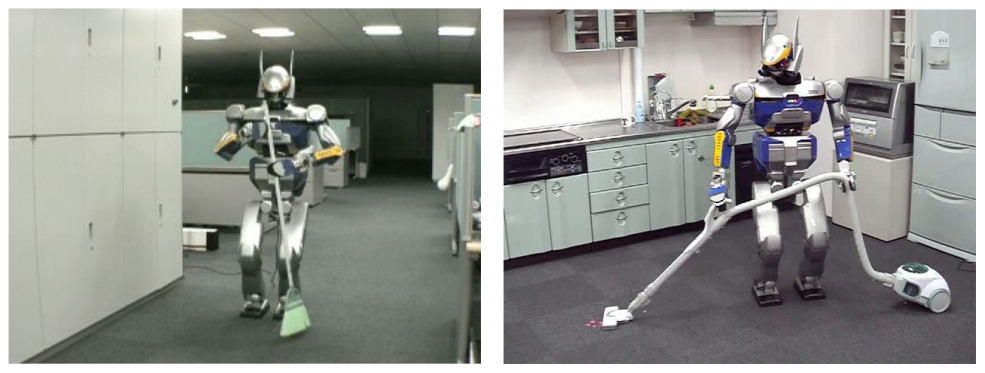
\includegraphics[width = 0.7\textwidth]{okada2006_1.png}
	\caption{Multi-purpose cleaning robot \cite{okada2006}.}
	\label{fig:okada2006_1}
\end{figure}

\section{Vacuum Robots}
\label{sec:vacuum_robots}

Comparing to other domestic chores, floor vacuuming is more challenging. In other tasks, \eg, cleaning of pool, solar panel or window, the robots usually handle static and known space. The environment is mostly two-dimensional, sometimes requires fixed obstacle avoidance. Vacuum robots have to deal with more diverse environment settings, \eg, unknown map, dynamic obstacles, interaction with human. In addition, many customers lack willingness to make physical changes to their rooms for the robots \cite{vaussard2014ras}.

\subsection{Design Characteristics}
Early 2000s, some major ground works on coverage problem were laid down \cite{huang1986icra, zelinsky1993icar, choset2000ar, gabriely2002icra}. Before the end of 2005, many major companies released their first models of domestic cleaning robots \cite{siciliano2016}. Most of these models and even current ones still have a lot in common:
\begin{itemize}
	\setlength\itemsep{0em}
	\item Shape: Round-shaped
	\item Dimension: Varies in height, diameter around 30-40 cm
	\item Cleaning technology: One suction pump (as the main \ac{EE} tool) and side brush (as supporting tool)
	\item Common sensors: Sonar, bumper and cliff (stair avoidance) sensors
	\item Coverage strategy: Bang and bounce (random motion), contour following
\end{itemize}

Most early models have round shape. The suction pump is limited between the two wheels. Another used design is D-shaped robot (\figref{fig:neato}), enabling wider brush and more corner coverage.

\begin{figure}[!htb]
	\centering
	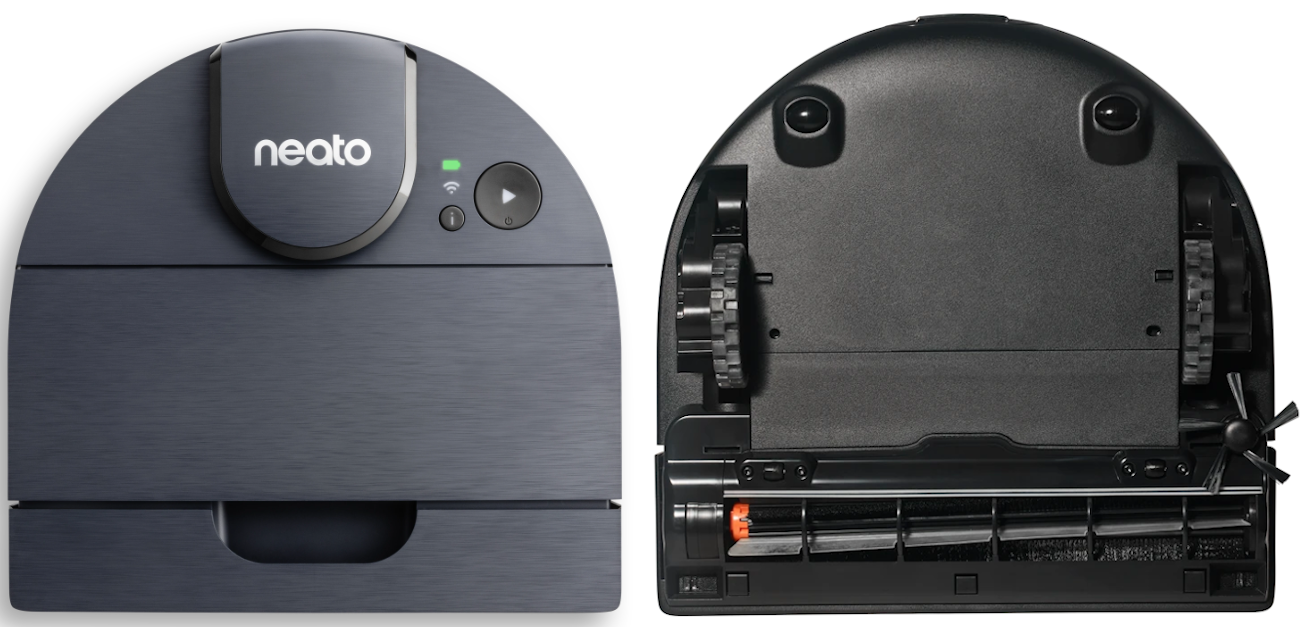
\includegraphics[width = 0.55\textwidth]{neato.png}
	\caption{Neato Robotics: Neato D8 \cite{neato}.}
	\label{fig:neato}
\end{figure}

Even though it is better to have knowledge of surrounding environment, domestic robots generally have the minimum amount of sensors. A \$20 sensor is very expensive for a robot that should cost around \$300-400. However, there are still exceptional cases. Costing \$3400 , Ottoro has two digital cameras, 12 pairs of ultrasonic sensor and highly sensitive air bumper (\figref{fig:ottoro}). With all state-of-the-art technologies, the robot could identify its position with the accuracy of $\pm$3cm and follow better coverage strategies. \cite{siciliano2016}

\begin{figure}[!htb]
	\centering
	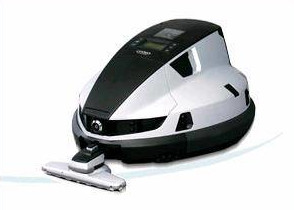
\includegraphics[width = 0.4\textwidth]{ottoro.jpg}
	\caption{Hanool Robotics: Ottoro \cite{ottoro}.}
	\label{fig:ottoro}
\end{figure}

Early robot models use simple approaches to coverage problem, \ie, \textit{Bang and Bounce}. With only a bumper sensor at the front, this strategy changes the robot direction whenever it hits an obstacle. Despite not guaranteeing complete coverage, this strategy converges to good space coverage after a large amount of time (\figref{fig:liu2008wcica_1}) \cite{liu2008wcica}. Some models integrate with contour following, achieved by adding sensor on the robot side for wall detection. As users are expecting more intelligent robots, a random motion is hardly appealing any longer \cite{goel2013iros}.

\begin{figure}[!htb]
	\centering
	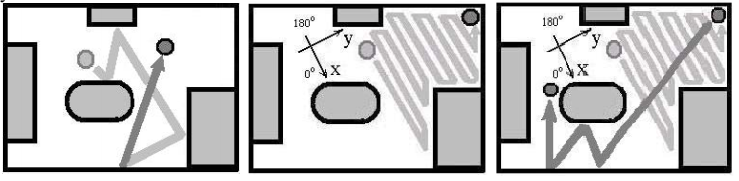
\includegraphics[width = 0.7\textwidth]{liu2008wcica_1.png}
	\caption{Random and fixed motion mode \cite{liu2008wcica}.}
	\label{fig:liu2008wcica_1}
\end{figure}

\subsection{Cost}
Whether a cleaning robot would be a business success or failure depends heavily on its cost. Early models, with the costs from \texteuro 800-1750, were 10-20 times more expensive than a high-quality vacuum cleaner. Despite the high cost, many were frequently trapped by electrical cables and need monthly repairs. This led to the lack of trust from customers in the autonomy of these robots \cite{vaussard2014ras}. The first robot successfully entering the domestic market was Roomba from iRobot. Its success was not due to its performance, rather the affordable price, \ie \texteuro 350. To take advantage of this market potential, next generation robots should consider not only engineering improvements, but also customer perceptions. \cite{gutmann2012arso, royakkers2015ijsr, siciliano2016}

\section{Coverage Path Planning}

\subsection{Introduction}

\ac{CPP} is the problem of finding the most optimal path to fully cover an area. Given a robot description and a map to cover, the output is a robot trajectory. \citeausm{huang1986icra} first describe the problem and its usage for robotic lawnmowers. Early seminal works formalize the coverage problem and propose new algorithms that prioritize coverage completeness \cite{latombe1991, zelinsky1993icar, choset2000ar}. In recent years, researchers have focused on other aspects of the coverage problem, \eg, extending it to dynamic or 3D environments, accounting for kinematic constraints, planning for several robots.\\

One application of coverage algorithm is for vacuum robots, which has huge business potential \cite{schofield1995, ifr}. The market is currently very competitive with many technological innovations and diverse robot approaches. Traditional round-shaped robot models are easy with to plan with, but have trouble cleaning along the floor edges and corners thoroughly. Other products try to clean better along the edges by resorting to a D-shaped robot, although it is more difficult to navigate with.\\

In practice, two issues often arise when planning coverage paths that have often been abstracted away in the literature: the need to account for the precise robot shape with \ac{EE} placement, and a lack of unified metrics for algorithm performance. My thesis examines in details these two issues for robot with asymmetric \ac{EE}.\\

\subsection{Classification}

Classification of \ac{CPP} takes form in many criteria, the most common ones and their corresponding classes are as follows:

\begin{itemize}
	\item Based on problem characteristics:
	\begin{itemize}
		\item Offline or Online: Offline algorithm assumes full prior knowledge of a static environment. Online algorithm do not make that assumption. As most online approaches utilize data from real-time sensor, they are also known as sensor-based coverage algorithms.
		\item With or without kinematics constraints: whether the robots could easily rotate in place or have a minimum turn radius.
	\end{itemize}
	\item Based on solution characteristics:
	\begin{itemize}
		\item Heuristics or Complete: whether the algorithms guarantee complete coverage of space.
		\item Type of environment decomposition: exact, approximate or semi-approximate cellular decomposition.
	\end{itemize}	
\end{itemize}

This subsection introduces some well-known coverage approaches.

\subsubsection{Trapezoidal Decomposition \ac{CPP}}
\citeaus{latombe1991} introduces the simplest offline exact cellular decomposition for 2D map. He assumes that map and obstacles are polygonal. When touching a obstacle vertex point, the swiping line divides the map into trapezoidal cells. One downside of this decomposition approach is to generate some redundant cells. \Eg, in \figref{fig:galceran2013ras_1}, the 9th and 11th cells can be grouped to one single cell. The less nodes there are, the easier it is to solve the associated \ac{TSP}.

\begin{figure}[!htb]
	\centering
	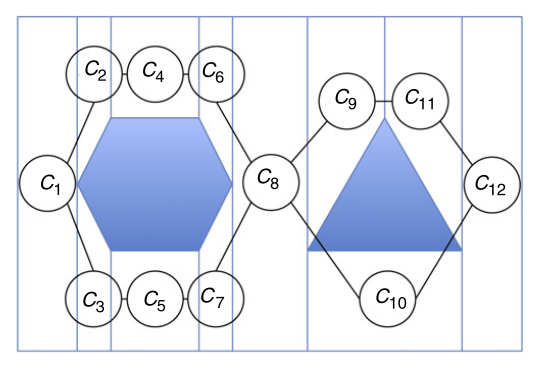
\includegraphics[width = 0.5\textwidth]{galceran2013ras_1.png}
	\caption{Trapezoidal decomposition with polygonal space and obstacles \cite{galceran2013ras}.}
	\label{fig:galceran2013ras_1}
\end{figure}

\subsubsection{Boustrophedon Decomposition \ac{CPP}}
\citeaus{choset2000ar} reduces the number of unnecessary cells. New cells are created only in an \textit{event}, when a cell is split into many or when cells are merged into one (\figref{fig:choset2000ar_1}). In such \textit{event}, the intersection point between the swiping line and obstacle boundary is a \textit{critical point}. The word \textit{boustrophedon} implies the simple zig-zag coverage pattern. The author also notes that using boustrophedon pattern alone is prone to incomplete coverage. The robot specifically misses areas around the obstacle perimeters, which are not parallel to the moving direction.

\begin{figure}[!htb]
	\centering
	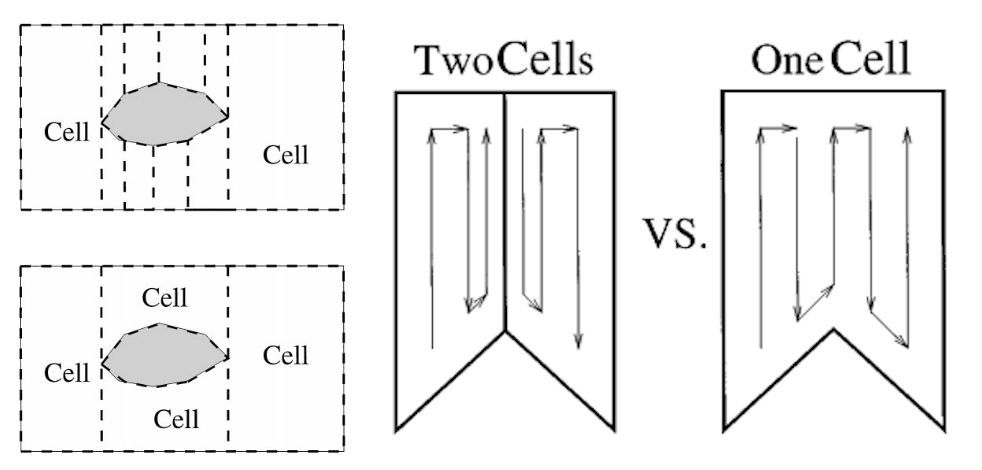
\includegraphics[width = 0.7\textwidth]{choset2000ar_4.png}
	\caption{Having less cells by creating new ones only in split or merge event.}
	\label{fig:choset2000ar_1}
\end{figure}

\subsubsection{Decomposition in terms of Critical Points of Morse Functions}
Previous presented approaches decompose the map using a line. \citeausm{choset2000icra} generalize the shape of the slice by changing its functional definition, called Morse function. For Boustrophedon Decomposition, the slice function of a line is $h(x)=x$, where $x$ is the first coordinate in 2D space. Different Morse functions induce different cell shapes and their corresponding coverage patterns (\figref{fig:choset2000icra_1}). Different problem settings may fit better with one coverage pattern than the others. \citeaus{acar2001iros} later develop an online \ac{CPP} algorithm using Morse function based decomposition.

\begin{figure}[!htb]
	\centering
	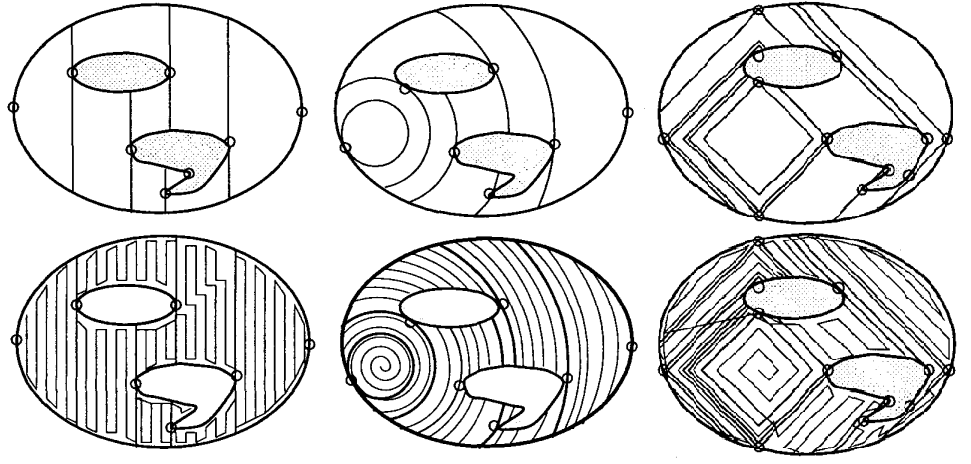
\includegraphics[width = 0.7\textwidth]{choset2000icra_1.png}
	\caption{Boustrophedon, spiral, diamond cell decompositions and coverage patterns~\cite{choset2000icra}.}
	\label{fig:choset2000icra_1}
\end{figure}

\subsubsection{Wavefront \ac{CPP} Algorithm}
\citeausm{zelinsky1993icar} use a completely different branch of approaches to CPP. They adopt their approach for \ac{PP} problem \cite{zelinsky1991}, to create a numeric potential field over the map using the distance transform. The distance wave increases in value as it spreads from goal point to neighbouring grid cells, until every cell is reached. If the robot follows a gradient-descent path, it is the shortest path from start to end point. On the other hands, if the robot follows a gradient-ascent path, it visits all cells and covers the whole map (\figref{fig:zelinsky1993_2}). To reduce high number of turns in \textit{distance transform}, the authors propose to add the distance from walls and obstacles to the potential field, resulting the \textit{path transform} trajectory. The approach is offline and allows start and end points to be specified.

\begin{figure}[!htb]
	\centering
	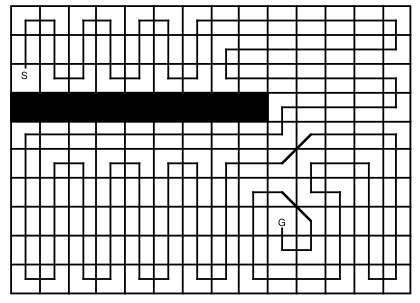
\includegraphics[width = 0.5\textwidth]{zelinsky1993_2.png}
	\caption{Complete coverage path.}
	\label{fig:zelinsky1993_2}
\end{figure}

\subsubsection{Spiral-STC Grid-based \ac{CPP} Algorithm}
\citeaus{gabriely2002icra} propose an online algorithm guaranteeing complete coverage of all free accessible subcells. They first divide the map into large cells, and each one of them contains four small subcells. At each position, the robot explores neighbouring large cell in a certain direction (counter clockwise). As large cells are visited, the spanning tree connecting them extends a new branch. This process iterates until the robot visits all possible large cells. In this exploration stage, the robot has travelled only on one side of the spanning tree. Then, the robot turns back and traverses on the other side of the tree to cover the rest of the map (\figref{fig:gabriely2002icra_2}).

\begin{figure}[!htb]
	\centering
	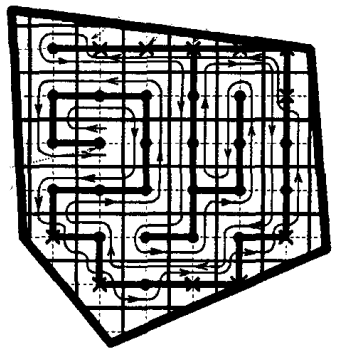
\includegraphics[width = 0.35\textwidth]{gabriely2002icra_2.png}
	\caption{An execution of full Spiral-STC.}
	\label{fig:gabriely2002icra_2}
\end{figure}

\subsubsection{Neural Network Approach to CPP}
The online \ac{CPP} approach by \citeaus{yang2004tsmc} is inspired by neural networks. Each cell in the grid map also represents a neuron in the network. The receptive field of each cell is only its 8 neighbours. Each neuron has a shunting dynamic equation. Certain thresholds over the shunting inputs allow the positive neural activities (pull activities from free spaces) to spread across the map, while limit the negative neural activities (push activities from obstacles) to stay in each local area. To limit the number of turns, the robot path takes both neural activity and previous poses into account. In the end, it also results in a potential field, similar to the one in \citeauthor*{zelinsky1993icar}'s work (\figref{fig:yang2004_3}). This approach can deal with dynamic and unstructured obstacles. However, unlike other online algorithms, \eg, \cite{butler2000, acar2001iros, gabriely2002icra}, for the network setup, the map size must be known a priori.

\begin{figure}[!htb]
	\centering
	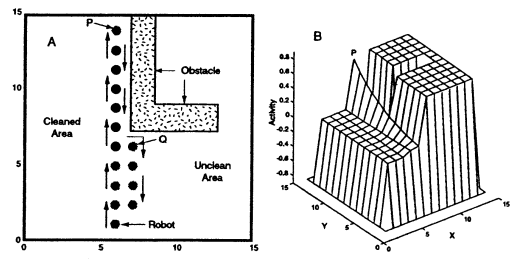
\includegraphics[width = 0.7\textwidth]{yang2004_3.png}
	\caption{Robot path and the activity landscape \cite{yang2004tsmc}.}
	\label{fig:yang2004_3}
\end{figure}

\subsubsection{Convex Sensor Placement Problem to \ac{CPP}}
\citeausm{arain2015icra} solve the convex sensor placement problem by formulating a novel directed graph on top of the grid map. Each cell has four nodes, corresponding to four poses. Each node has connections with other nodes in the same grid cell and one node in the neighbouring cell of the same direction. \Eg, if the current node represents the pose going up, it connects with the node going up in the above grid cell, if that exists (\figref{fig:arain2015icra_1}). As an area inspection problem, the range of the end-effector (a gas detection sensor) is much greater than the size of each grid cell. The coverage problem is similar to the \ac{CSP}, which doesn't require to visit all nodes in the graph. The authors find a path traversing the graph using iterative convex relaxation method (\figref{fig:arain2015icra_2}).

\begin{figure}[!htb]
	\centering
	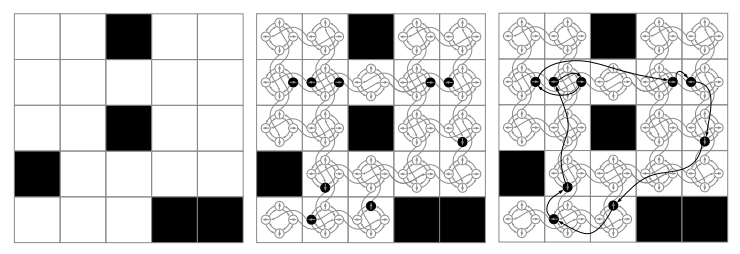
\includegraphics[width = 1\textwidth]{arain2015icra_2.png}
	\caption{Trajectory from traversing the graph.}
	\label{fig:arain2015icra_2}
\end{figure}

\subsubsection{Turn-minimizing Coverage}
The offline algorithm of \citeaus{vandermeulen2019icra} resembles the line-sweep-based decomposition \cite{huang2001icra}, but for grid-based approach. The authors consider the problem as a \ac{TSP} instance. A \textit{rank} is similar to a sweep line and is a node in the \ac{TSP}. The robot covers the map by visiting all interior and perimeter ranks (\figref{fig:vandermeulen2019icra_5}). Each rank has three vertices: two end points and a midpoint. As the cost from the midpoint vertex to vertices in other ranks is infinity, it enforces the robot to go from one end to the others within a rank.

\begin{figure}[!htb]
	\centering
	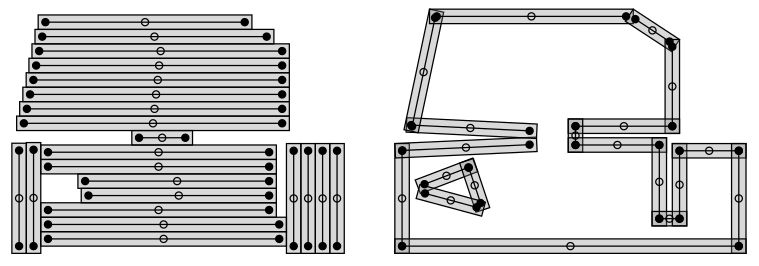
\includegraphics[width = 0.79\textwidth]{vandermeulen2019icra_5.png}
	\caption{Interior and perimeter ranks. \cite{vandermeulen2019icra}.}
	\label{fig:vandermeulen2019icra_5}
\end{figure} 

\clearpage
% !TeX spellcheck = en_US
\chapter{Conclusion}

The internship at the Bosch CR/AAS3 department was my first experience in a large and professional company. It opens up my point of view about the complete process of software development. I still have many gaps of knowledge to fill, but unlike before, I have more awareness of the direction to follow. During the internship, I mainly code and work with software. The Corona situation made it harder to work and cooperate with others. Regardless, it was a great opportunity, allowing me to learn, experience and prepare for the future.


\pagenumbering{Roman}
\printbibliography[heading=bibintoc]

\end{document}